%% This is file `elsarticle-template-1-num.tex',
%% %% Copyright 2009 Elsevier Ltd
%%
%% This file is part of the 'Elsarticle Bundle'.
%% ---------------------------------------------
%%
%% It may be distributed under the conditions of the LaTeX Project Public
%% License, either version 1.2 of this license or (at your option) any
%% later version.  The latest version of this license is in
%%    http://www.latex-project.org/lppl.txt
%% and version 1.2 or later is part of all distributions of LaTeX
%% version 1999/12/01 or later.
%%
%% The list of all files belonging to the 'Elsarticle Bundle' is
%% given in the file `manifest.txt'.
%%
%% Template article for Elsevier's document class `elsarticle'
%% with numbered style bibliographic references
%%
%% $Id: elsarticle-template-1-num.tex 149 2009-10-08 05:01:15Z rishi $
%% $URL: http://lenova.river-valley.com/svn/elsbst/trunk/elsarticle-template-1-num.tex $
%%

%\documentclass[]{article}
\documentclass[preprint,3p,12pt]{elsarticle}
%\documentclass[final,5p,times,twocolumn]{elsarticle}

%% Use the option review to obtain double line spacing
%% \documentclass[preprint,review,12pt]{elsarticle}

%% Use the options 1p,twocolumn; 3p; 3p,twocolumn; 5p; or 5p,twocolumn
%% for a journal layout:
%% \documentclass[final,1p,times]{elsarticle}
%% \documentclass[final,1p,times,twocolumn]{elsarticle}
%% \documentclass[final,3p,times]{elsarticle}
%% \documentclass[final,3p,times,twocolumn]{elsarticle}
%% \documentclass[final,5p,times]{elsarticle}
%% \documentclass[final,5p,times,twocolumn]{elsarticle}

\usepackage{amssymb}
\usepackage{wrapfig}
\usepackage{lipsum}
\usepackage{natbib}

\usepackage{tikz}
\usepackage{mathdots}
\usetikzlibrary{shapes, arrows}

\usepackage{graphicx}
\graphicspath{ {./graphics/} }


%% Styles for proximity flow chart
\tikzstyle{ccell} = [rectangle, draw, fill=red!20, minimum width=3em, text centered, minimum height=3em]
\tikzstyle{dcell} = [rectangle, draw, fill=brown!20, minimum width=3em, text centered, minimum height=3em]
\tikzstyle{gcell} = [rectangle, draw, fill=yellow!20, minimum width=3em, text centered, minimum height=3em]
\tikzstyle{fcell} = [rectangle, draw, fill=green!20, minimum width=3em, text centered, minimum height=3em]
\tikzstyle{ucell} = [rectangle, draw, fill=white!20, minimum width=3em, text centered, minimum height=3em]
\tikzstyle{line} = [draw, -latex']


\journal{University of Guelph; CIS*4780}

\begin{document}

\begin{frontmatter}

\title{Two Dimensional Intelligent Character Recognition}


\author[ryan,doug,oliver]{Ryan Pattison, Douglas Anderson, and Oliver Cook}
\address[ryan]{ryan.m.pattison@gmail.com}
\address[doug]{dander01@uoguelph.ca}
\address[oliver]{cooko@uoguelph.ca}


\begin{abstract}

For quite some time computer vision has been used to extract characters from
images in order to gain knowledge from text. In recent years many of the
techniques for recognizing characters has been based on machine learning.


\end{abstract}

\begin{keyword}
% keywords here, in the form: keyword \sep keyword
Machine Learning \sep
Data Mining \sep
Computer Vision \sep
Intelligent Character Recognition
\end{keyword}

\end{frontmatter}

\section{Introduction}
\label{intro}


The problem of Intelligent Character Recognition (ICR) in Artificial
Intelligence and Machine Learning has received much attention in past years.
This field of study has focused on the classification of \emph{handwritten}  or
\emph{typewritten} letters and numbers.  The novelty of this project will be in
the development of an algorithm which recognizes characters, or more generally
symbols, arranged to form words in \emph{two} dimensions. The practical
application proposed here will be the development of an algorithm for
recognizing hand drawn cartography. To this end, we have defined a small set of
symbols to represent various terrains: grass, mountains, bodies of water, and
more. Each symbol will be drawn into a single cell on a standard sheet of grid
paper and scanned into a computer. Using the scanned images, several
algorithms will learn to recognize the symbols cell-by-cell as well as in the
context of the surrounding cells. In order to demonstrate
the utility of such an algorithm, we propose an application which reads a
hand drawn map and produces a computer generated image of the same map. To do this,
we will use the software tool WEKA\cite{hall2009} to assist us in the creation
of various classifiers.



\section{Process}
\label{process}

\subsection{Overview}
\label{process:overview}

\begin{figure}[h]
\begin{center}
\includegraphics[width=2in]{PokemonPalletTown.png}
\end{center}
\caption{Pallet Town map from Pok\'{e}mon\cite{firered}} 
\label{fig:pokemon}
\end{figure}

\begin{table}
\label{table:symbols}
\caption{Symbols Names and the Hand drawn equivalents}
\begin{center}
\begin{tabular}{llll}
Water & \includegraphics[width=.5in]{water.png} &
Grass & \includegraphics[width=.5in]{grass.png} \\
Rock & \includegraphics[width=.5in]{rocks.png} &
Tree & \includegraphics[width=.5in]{tree.png} \\
Dirt & \includegraphics[width=.5in]{dirt.png} &
Sand & \includegraphics[width=.5in]{sand.png} \\
\end{tabular}
\end{center}
\end{table}

We have created 6 symbols to be used to recreate maps for a popular video game
Pok\'{e}mon to ensure that our data set is sampled from a well defined distribution.
An example map from the game is shown in Figure \ref{fig:pokemon}. There is a sample
of the the symbols names and the hand drawn equivalents in Table \ref{table:symbols}.




\subsection{Preprocessing}
\label{process:preprocessing}


For all of our analysis we pre-process colour images images into black and white
images. To do this we first remove the blue grid lines from the image and
replace them with white. We then remove all colour information from the image
and resize it such that every cell of the grid is 75 pixels by 75 pixels.

\begin{figure}[h]
    \begin{center}
    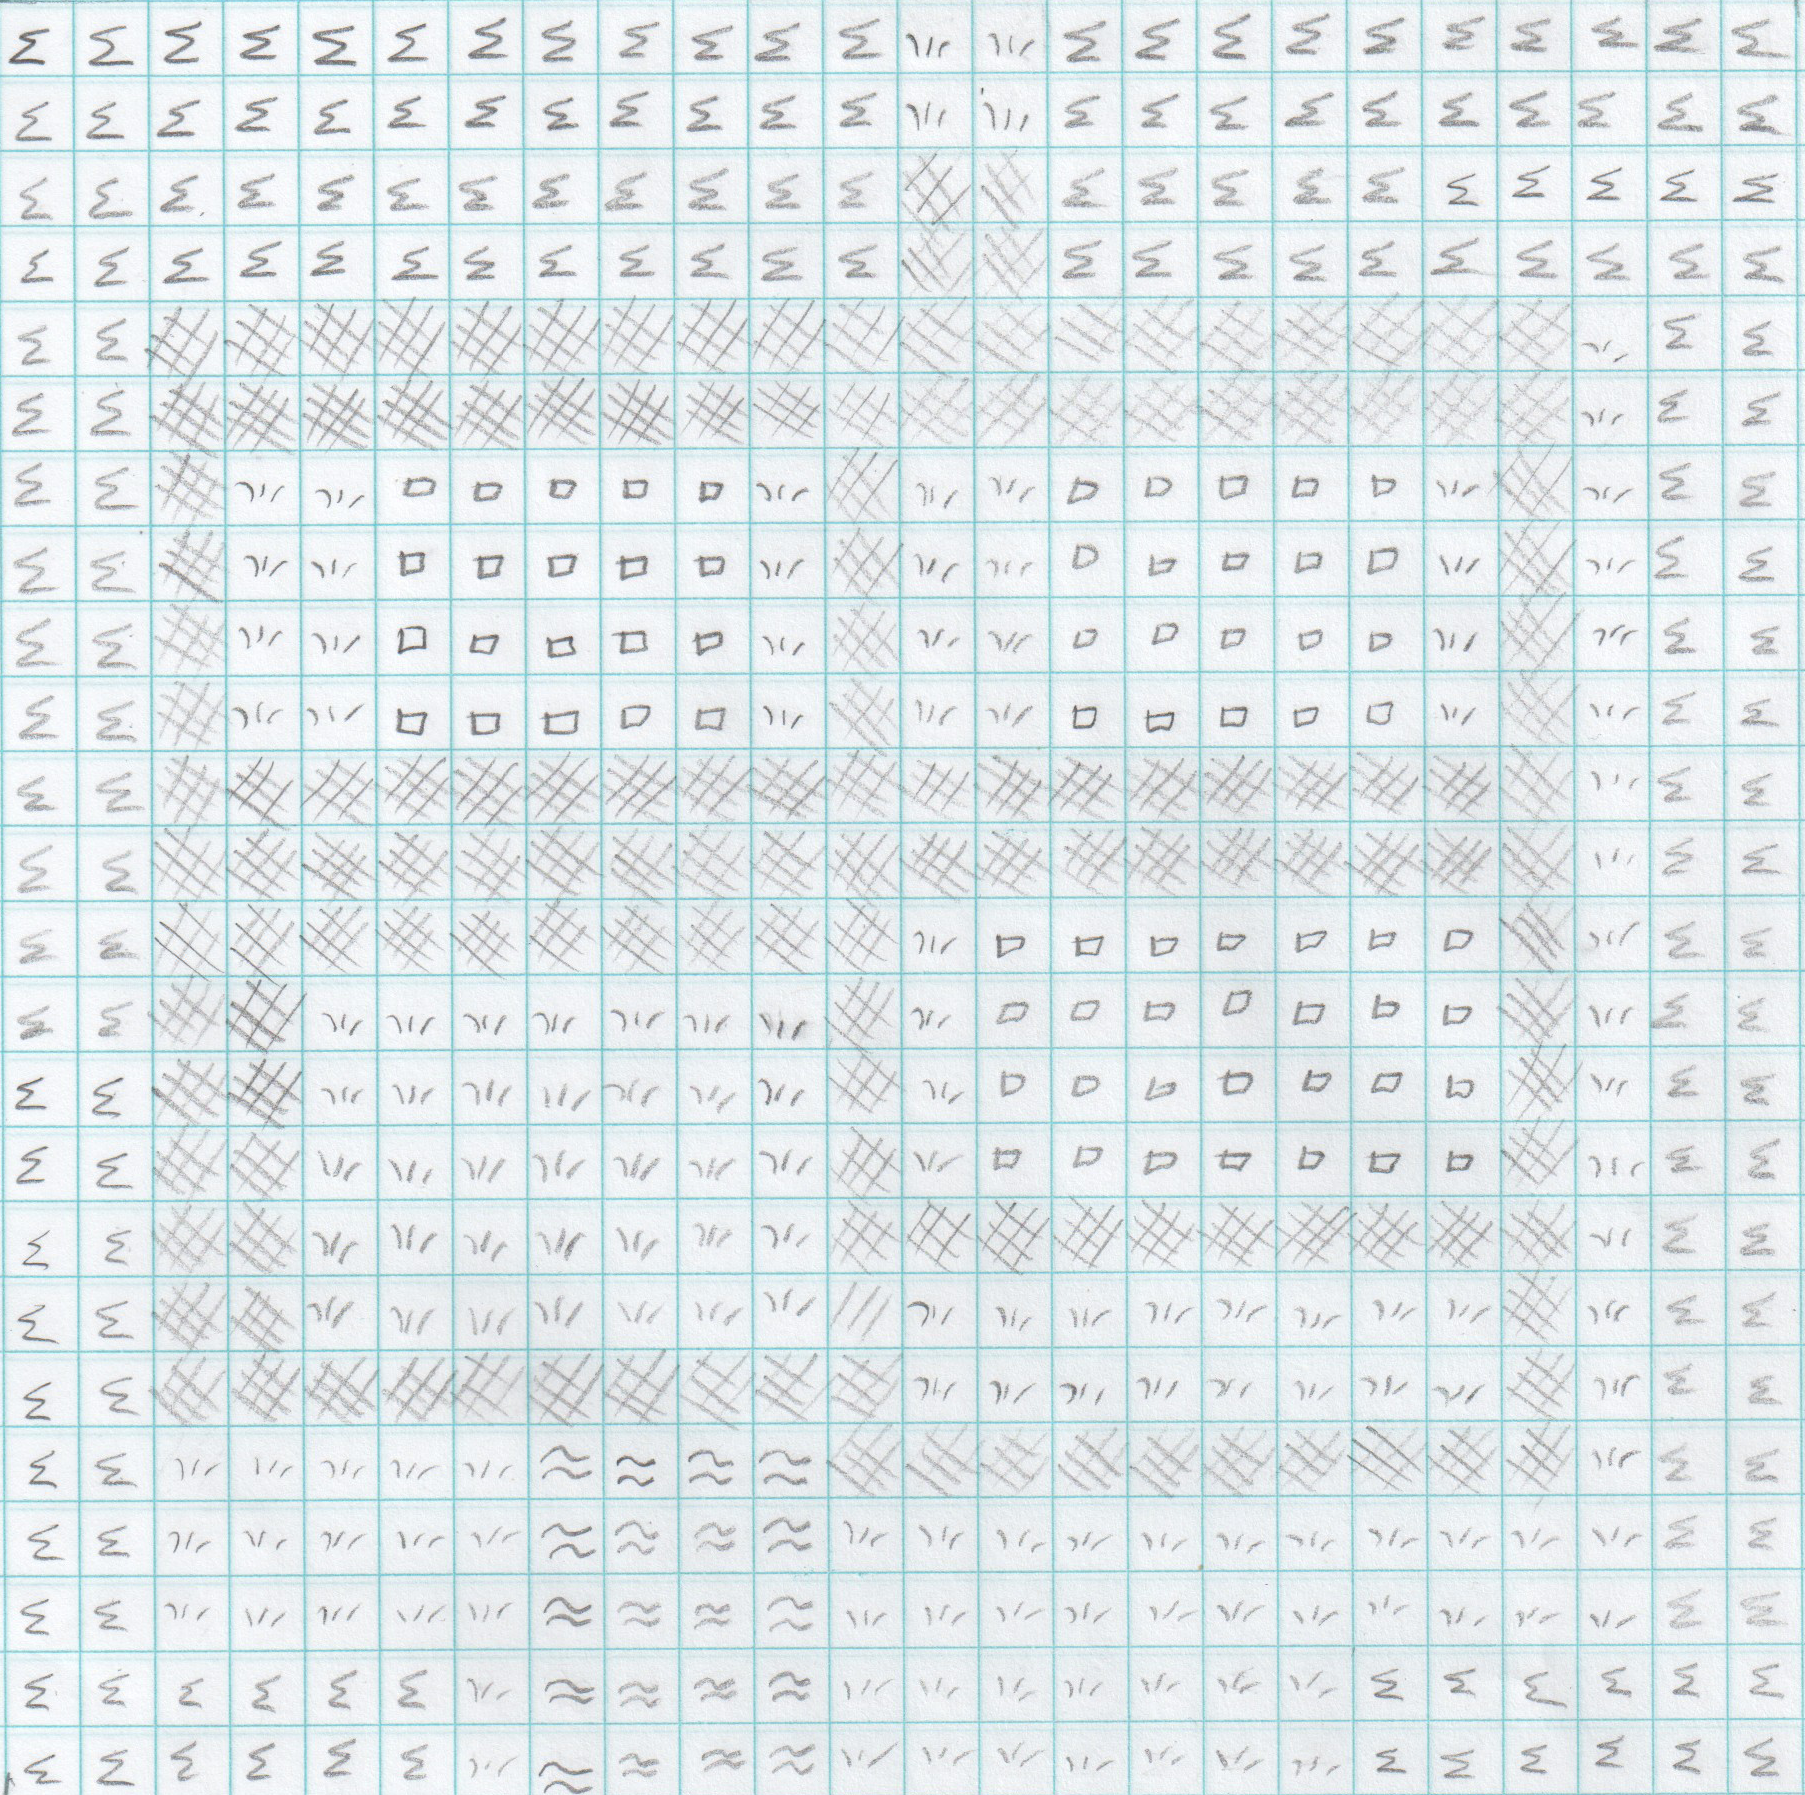
\includegraphics[width=7.5cm, height=7.5cm]{preprocessing-initial}
    \includegraphics[width=7.5cm, height=7.5cm]{preprocessing-final}

    \caption{Image before preprocessing and image after preprocessing. Notice
        that the contrast has increased and the blue lines have been partially
        removed}

    \end{center}
\end{figure}


\subsection{Feature-Based Approach}
\label{process:featurebased}


The feature based method is used to extract geometric information about the
shape and distribution of the points which make up the symbol. To extract these
features, the approach used here applies convolution filters to the cell images,
and then gathers statistics based on the distribution of black pixels in each
of the $x$ and $y$ dimensions. A convolution filter is a matrix of coefficients
and is of an odd size. The matrix is used to transform an image into another
image which may make certain attributes, such as edges, more prominent.  For
example, the convolution filter, $F_{blur}$ is a mean blur. The convolution
filter transforms the image by replacing each pixel with a new filtered pixel.
The new pixel is created by multiplying the surrounding values by those in the
convolution filter and summing the result, this sum is the new value for the
pixel.

\[ F_{blur} = \left[
\begin{array}{ccc}
1/16 & 2/16 & 1/16 \\
2/16 & 4/16 & 2/16 \\
1/16 & 2/16 & 1/16
\end{array}\right] \]

\begin{figure}[h] \[
\begin{array}{lcr}
\begin{array}{ccccc}
\ddots & \vdots & \vdots & \vdots & \iddots \\
\ldots & 64 & 64 & 32 & \ldots \\
\ldots & 32 & \fbox{32} & 128 & \ldots \\
\ldots & 32 & 16 & 32 & \ldots \\
\iddots & \vdots & \vdots & \vdots & \ddots \\
\end{array} &
\begin{array}{c}
64F_{11} + 64F_{12} + 32F_{13} \\
+ 32F_{21} + 32F_{22} + 128F_{23} \\
+ 32F_{31} + 16F_{32} + 32F_{32} \\
\end{array} &
\begin{array}{ccccc}
\ddots & \vdots & \iddots \\
\ldots &  \fbox{48}  & \ldots \\
\iddots & \vdots & \ddots \\
\end{array}
\end{array} \]
\caption{Applying the convolution filter to the centred pixel area}
\label{figure:convolution}
\end{figure}

A filtered image is created as the result of the convolution matrix being
applied to each pixel. Figure \ref{figure:convolution} shows the filter being
applied to a single pixel. The filtering process repeats for each pixel until
all pixels have been replaced qnd resulting image has a luminance matrix,
which we will call $A$.

\[A = \left [
    \begin{array}{r r r r}
        a_{00} & a_{10} & \cdots & a_{n0} \\
        a_{01} & a_{11} & \cdots & a_{n1}\\
        \vdots  & \vdots  & \ddots & \vdots\\
        a_{0m} & a_{1m} & \cdots & a_{nm}\\
    \end{array}
\right ] \]

We define $x$ and $y$ to be the row and column sum functions.

\begin{equation}
x(i) = \sum_{j}{A_{i,j}} \quad
y(j) = \sum_{i}{A_{i,j}}
\end{equation}

Next we record the means and standard deviations: $\mu_x, \mu_y, \sigma_x,
\sigma_y$ as the feature set for this filter. Then we apply another
filter, either on this filtered image or, on the original image and record
statistics on these as well.



\subsection{Gold Comparison Approach}


\begin{figure}[h]
\includegraphics{building-mean}
\includegraphics{dirt-mean}
\includegraphics{forest-mean}
\includegraphics{grass-mean}
\includegraphics{water-mean}
\includegraphics{rocks-mean}

\caption{The gold images created as the mean image of all examples of each symbol. In order we have symbols reprenting buildings, dirt, forest, grass, water, and rocks.}

\end{figure}

Similar to the Feature-based approach we define $x$ and $y$ to be the row and column sums and calculate the mean and standard deviation.
To get the symbols to overlap we apply a linear transformation to each pixel using the statistics gathered in each dimension.
\begin{equation} \label{eq:gold}
x^{\prime} = (x - \mu^{B}_{x}) \, \frac{\sigma^{G}_{x}}{\sigma^{C}_{x}} + \mu^{G}_{x} \quad
y^{\prime} = (y - \mu^{B}_{y}) \, \frac{\sigma^{G}_{y}}{\sigma^{C}_{y}} + \mu^{G}_{y}
\end{equation}

We then compare the overlapping image $A$ to the gold standard image $G$ by taking the sum of the squared difference at each pixel position.
This gives us an error measure which we record for each class $k$.

\[
\xi_{k}(A) = \sum_{i}\sum_{j}{(A_{ij} - G_{kij})^{2}}
\]

The result is a vector of size $k$, the number of classes, with an error measure for the comparison
against the corresponding class. We then input this vector into WEKA along with the correct answer
for training purposes. We used a J48 decision tree with 10-fold validation.


\subsection{Proximity Approach}
\label{process:proximity}


The proximity classifier learns the patterns of symbols present in the data set,
and then classifies any unknown symbols using the surrounding symbols, and its
knowledge of the patterns and relationships of the symbols. Here we begin by
outlining the methodology used; we want to classify the symbol $x$ at a given
position, as Figure~\ref{fig:neighbours} illustrates.

\begin{figure}[h]
\begin{center}
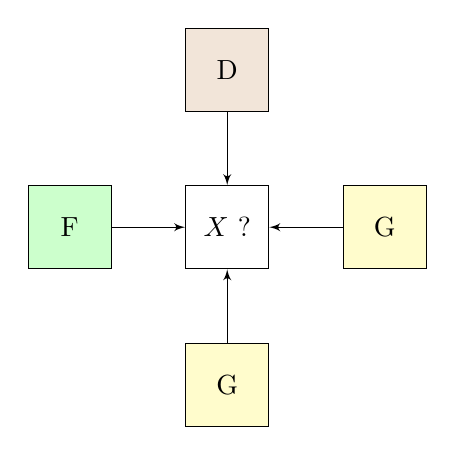
\begin{tikzpicture}[node distance=2cm, auto]
    \node[dcell](top){D};
    \node[ucell, below of=top](center){$X$~?};
    \node[fcell, left of=center](left){F};
    \node[gcell, right of=center](right){G};
    \node[gcell, below of=center](bottom){G};

    \path[line] (top)   -- node[right] {} (center);
    \path[line] (left)   -- node[above] {} (center);
    \path[line] (right)   -- node[above] {} (center);
    \path[line] (bottom)   -- node[right] {} (center);
\end{tikzpicture}
\end{center}
\caption{This example is from cell 2,19 in Pallet Town, Note: $G$=grass, $D$=dirt, $F$=forest}
\label{fig:neighbours}
\end{figure}


\begin{table}[h]
\label{table:relativefreq}
\begin{center}
\begin{tabular}{ l | r r r r r r }
              & $c_{B}$& $c_{D}$& $c_{EDGE}$& $c_{F}$& $c_{G}$& $c_{W}$ \\ 
              \hline
    north     & 0      & 0.1558 & 0.0519    & 0.0519 & 0.7403 & 0.0325\\
    east      & 0.0779 & 0.0974 & 0         & 0.1493 & 0.6428 & 0\\
    south     & 0      & 0.2403 & 0.0130    & 0.0065 & 0.7403 & 0\\
    west      & 0.0519 & 0.2273 & 0         & 0.0519 & 0.6428 & 0.0260\\
\end{tabular}
\caption{Probability of the neighbours for a grass cell in Pallet Town}
\end{center}
\end{table}

To classify x, we first calculate the probability that $x$ belongs to each
class, $P(X)\quad X_i = P(x\!\in\! C_i)$. The proximity classifier is given the
class of each symbol in the cardinal directions: north, south, east, and west.
Using this information, we restrict the probability calculation to consider
only the case where a symbol has the given classes neighbouring it. Such a
restriction is the conditional probability:

\[
P(X) = P(X|\,N\!=\!c_1,\,E\!=\!c_2,\,S\!=\!c_3,\,W\!=\!c_4)
\]

\begin{figure}[h]
\begin{center}
\begin{tikzpicture}[node distance=3cm, auto]
    \node[ccell](top){$C_{i,j+1}$};
    \node[ucell, below=of top](center){$X_{i,j}$};
    \node[ccell, left=of center](left){$C_{i-1,j}$};
    \node[ccell, right=of center](right){$C_{i+1,j}$};
    \node[ccell, below=of center](bottom){$C_{i,j-1}$};

    \path[line] (top)   -- node[above right] {$P(X | \, N=c_{1})$} (center);
    \path[line] (left)  -- node[above] {$P(X | \, W=c_{2})$} (center);
    \path[line] (right) -- node[above] {$P(X | \, E=c_{3})$} (center);
    \path[line] (bottom) -- node[below right] {$P(X | \, S=c_{4})$} (center);
\end{tikzpicture}
\end{center}
\caption{The conditional probability of the classes for $X_{i,j}$, given the neighbouring cells}
\label{fig:conditionalprob}
\end{figure}


In calculating probabilities, we can only approximate them using relative
frequencies collected from our sample data. For a set of $k$ classes, there are
$k^5$ possible combinations of cells, 4 neighbouring cells and the centre, and
too many of these combinations occur rarely in our dataset to make confident
approximations of the true probabilities. To resolve this problem, we assume
that the conditional probabilities are independent in each direction. Under
this assumption, the calculation becomes much more reasonable for our small
data set, since there are only $4k$ pieces of data to record for each symbol.
Our resulting calculation is given in Equation~\ref{eq:prox}.

\begin{equation}
\label{eq:prox}
P(X) \approx P(X|\,N\!=\!c_1)P(X|\,S\!=\!c_2)P(X|\,E\!=\!c_3)P(X|\,W\!=\!c_4)
\end{equation}

From the definition of conditional probability we have that for some class $c$ in
the direction $D$:
\[
P(X|\,D\!=\!c) = \frac{P(X \cap D\!=\!c)}{P(D=c)}
\]

To calculate each of the conditional probabilities, we compute a table from the
samples recording $P(X\cap D\!=\!c)$ and $P(D\!=\!c)$ for each class  $c$, and
direction $D$, an example is given for a single class in
Table~\ref{table:relativefreq}.  We use the table to calculate the relative
conditional frequencies and, under the assumption of independence, we
approximate $P(X)$ using Equation~\ref{eq:prox}.

Having the probability vector $P(X)$ we create an input file for WEKA.  This
file includes the probability vector, the neighbouring classes, and the class
of the symbol being classified for training. WEKA creates a decision tree which
is used to reduce the error in the probability calculation that is introduced
under the assumption of independence.



\subsection{Classifier Training}
\label{process:training}
Training was done using WEKA and 10-fold cross validation.
the proximity classifier was tested on a map it had never seen in training.

\section{Results}
\label{results}


\begin{tabular}{lrlrrr}
Algorithm & Samples & Feature Set & Success & Features & Tree nodes \\
\hline
Feature-Based   & 9888  & Single Filter & 76.32 &  32 & ? \\
Feature-Based   & 9888  & No Spatial    & 80.64 & 205 & 1131 \\
Feature-Based   & 9888  & Spatial       & 82.47 & 207 & 1005 \\
Proximity       & 13200 & Surrounding   & 93.78 &  11 & ? \\ 
Gold Comparison & 225   & Probabilities & 70.40 &   7 & ? \\
Gold Comparison & 225   & Probabilities & 83.33 &   7 & ? \\
\end{tabular}



\section{Conclusions}
\label{conclusions}

Each of our classification methods each have their own strengths and
weaknesses.  The \textbf{Feature-Based method} is able to recognize arbitrary
features but requires intended representations of each of the maps during
training. \textbf{Proximity method} works extremely well with the set of maps
we chose because they adhere to patterns. However to detect these patterns in a
data set the proximity classifier needs a relatively accurate representation of
the map. This method has the added benift of haveing it's output be the same as
it's input.  The \textbf{Gold Comparison} method is able to classify symbols
fairly well without intended representations of the map. However this method
requires gold images as input and the number of features in the output
generated is dependent on the number of gold images.

We believe that for the best results the methods should be used in conjunction.
For example using the gold comparison method we could generate a decent
representation of the map which could then be cleaned up by the Proximity
method.


\section{Further Work}
\label{further work}


Future work may include combining the proximity classifier with the gold 
comparison classifier to improve accuracy. 

Feature based classification may see improvement from considering other
transformations of the pixels when calculating statistics, such as distance
from the centre.

Non mean golds

Regions with the feature extraction method


\section{References}
\label{references}


\bibliographystyle{plain}
\bibliography{report}


\end{document}

